\chapter{Analisa}

Pada bab ini, akan dilakukan analisa terhadap data yang akan diproses menggunakan \textsl{data mining} dan perangkat lunak yang akan dibangun untuk melakukan proses data tersebut.

\section{Analisis Data}
Pada bab ini, akan dilakukan analisa \textsl{preprocessing data} yang meliputi \textsl{data cleaning}, \textsl{data integration}, \textsl{data selection} dan \textsl{data transformation}. Setelah membaca dan menganalisis data \textsl{log} histori KIRI, maka penelitian ini akan lebih fokus untuk meneliti mengenai lokasi keberangkatan dan tujuan dari user yang menggunakan aplikasi KIRI.

\subsection{Data Cleaning}
Pada tahap ini, data yang akan menjadi input akan diperiksa apakah mengandung \textsl{missing value} atau \textsl{noisy}. Setelah dilakukan pemeriksaan, tidak ditemukan \textsl{missing value} ataupun \textsl{noisy}, sehingga tahap ini dapat dilewat.

\subsection{Data Integration}
Pada tahap ini, data-data dari beberapa database akan digabung dan diintegrasikan menjadi satu database. Karena data yang digunakan hanya berasal dari satu tabel, maka tahap ini dapat dilewat.

\subsection{\textsl{Data Selection}}
Pada tahap ini, akan dilakukan pemilihan data yang akan digunakan. Pada penelitian ini, akan dilakukan proses \textsl{data mining} mengenai lokasi keberangkatan dan tujuan dari seorang user yang menggunakan aplikasi KIRI. Oleh karena itu, pada atribut \textsl{action}, nilai yang akan dipilih hanya \textsl{FINDROUTE}. Hal ini dikarenakan, hanya \textsl{action FINDROUTE} yang menjelaskan posisi keberangkatan dan tujuan dari user. Selain itu, data tersebut terlihat menarik karena dimungkinkan dapat menghasilkan suatu pola yang membantu melakukan klasifikasi mengenai perpindahan penduduk khususnya untuk daerah Bandung. Karena seluruh \textsl{action} bernilai satu jenis yaitu \textsl{FINDROUTE}, maka atribut tersebut dapat dihilangkan. Selain itu, atribut logId dan APIKey tidak akan dimasukan ke dalam proses karena tidak memiliki hubungan dengan lokasi keberangkatan dan tujuan dari seorang user.

Dari analisis diatas, maka atribut yang dipilih untuk diproses ke dalam \textsl{data mining} adalah
\begin{itemize}
	\item \textsl{Timestamp} (UTC)
	\item \textsl{AdditionalData}
\end{itemize}

Berikut contoh data dari atribut tersebut dapat dilihat pada tabel 3.1
\begin{table}[h]
\caption{Contoh data \textsl{log} KIRI setelah \textsl{data selection}}
\begin{tabular}{|l|l|}
\hline
\textbf{Timestamp (UTC)} & \textbf{AdditionalData}                     \\ \hline
2/1/2014 0:11            & -6.8972513,107.6385574/-6.91358,107.62718/1 \\ \hline
2/1/2014 0:13            & -6.8972513,107.6385574/-6.91358,107.62718/1 \\ \hline
2/1/2014 0:16            & -6.90598,107.59714/-6.90855,107.61082/1     \\ \hline
2/1/2014 0:18            & -6.9015366,107.5414474/-6.88574,107.53816/1 \\ \hline
2/1/2014 0:25            & -6.90608,107.61530/-6.89140,107.61060/2     \\ \hline
2/1/2014 0:27            & -6.89459,107.58818/-6.89876,107.60886/2     \\ \hline
2/1/2014 0:28            & -6.89459,107.58818/-6.86031,107.61287/2     \\ \hline
\end{tabular}
\end{table}

Pada atribut \textsl{additionalData}, jika nilai atribut \textsl{action} adalah \textsl{FINDROUTE}, maka nilai \textsl{addtional data} memiliki tiga bagian yang dibatasi dengan '/'. Ketiga bagian tersebut adalah

\begin{enumerate}
	\item Nilai latitude dan longitude dari lokasi keberangkatan yang dipilih oleh user
	\item Nilai latitude dan longitude dari lokasi tujuan yang dipilih oleh user
	\item Nilai yang menunjukkan banyak jalur yang dihasilkan oleh sistem KIRI
\end{enumerate}

Nilai dari banyak jalur akan dibuang ketika memasuki tahap \textsl{data transformation}, karena nilai tersebut hanya menunjukkan banyak jalur tetapi user pasti hanya memilih salah satu dari jalur tersebut, sehingga nilai jalur ini dapat diasumsikan memiliki nilai 1 semua. karena kolom jalur bernilai satu semua, maka kolom tersebut dapat dibuang.

\subsection{\textsl{Data Transformation}}
Pada tahap ini, akan dilakukan perubahan data. Pada atribut yang dipilih, nilai dari atribut \textsl{timestamp} dan \textsl{additionaldata} perlu dilakukan transformasi agar program dapat membaca dan memproses data lebih cepat. 

Pada atribut \textsl{timestamp}, nilai waktu dari atribut tersebut akan diubah menjadi waktu GMT+8. Kemudian, data akan diubah menjadi enam atribut, yaitu:
\begin{itemize}
	\item Tanggal, atribut ini akan menunjukkan tanggal ketika user KIRI memanggil \textsl{action FINDROUTE}, dengan nilai antara 01 sampai 31
	\item Bulan, atribut ini akan menunjukkan bulan ketika user KIRI memanggil \textsl{action FINDROUTE}, dengan nilai antara 01 sampai 12 
	\item Tahun, atribut ini akan menunjukkan tahun ketika user KIRI memanggil \textsl{action FINDROUTE}, dengan format empat angka (contoh: 2014)
	\item Hari, atribut ini akan menunjukkan hari ketika user KIRI memanggil \textsl{action FINDROUTE}, dengan range nilai antara senin sampai minggu
	\item Jam, atribut ini akan menunjukkan jam ketika user KIRI memanggil \textsl{action FINDROUTE}, dengan range nilai antara 00 sampai 23
	\item Menit, atribut ini akan menunjukkan menit ketika user KIRI memanggil \textsl{action FINDROUTE}, dengan range nilai antara 00 sampai 59
\end{itemize}

Data \textsl{timestamp} diubah menjadi lima bagian, agar dapat dilakukan pengelompokan yang dilihat dari tanggal, bulan, tahun, hari, dan jam atau hasil dari \textsl{decision tree} dapat menghasilkan node yang menentukan tanggal, bulan, tahun, hari dan jam.

Pada atribut \textsl{additionalData}, data akan diubah menjadi empat atribut, yaitu:
\begin{itemize}
	\item Latitude keberangkatan, atribut ini berisi nilai latitude dari lokasi keberangkatan yang dipilih oleh user
	\item Longitude keberangkatan, atribut ini berisi nilai longitude dari lokasi keberangkatan yang dipilih oleh user
	\item Latitude tujuan, atribut ini berisi nilai latitude dari lokasi tujuan yang dipilih oleh user
	\item Longitude tujuan, atribut ini berisi nilai longitude dari lokasi tujuan yang dipilih oleh user
\end{itemize}

Data \textsl{additionalData} diubah menjadi empat bagian, agar program dapat membaca data tersebut lebih mudah.

Dari analisis diatas, banyak atribut dari tabel \textsl{statistics} akan menjadi sepuluh, yaitu:
\begin{itemize}
	\item Tanggal
	\item Bulan
	\item Tahun
	\item Hari
	\item Jam
	\item Menit
	\item Latitude Keberangkatan
	\item Longitude Keberangkatan
	\item Latitude Tujuan
	\item Longitude Tujuan
\end{itemize}

Contoh hasil data transformasi jika input merupakan data dari tabel 3.1 dapat dilihat pada tabel 3.2.

\begin{table}[h]
\caption{Contoh hasil data transformasi}
\begin{longtable}{|l|l|l|l|l|l|l|l|l|l|}
\hline
\textbf{Tanggal}	& \textbf{Bulan}	& \textbf{Tahun} 	& \textbf{Hari} & \textbf{Jam}	& \textbf{Menit} & \textbf{Latitude Keberangkatan} & \textbf{Longitude Keberangkatan} & \textbf{Latitude Tujuan} & \textbf{Longitude Tujuan}      \\ \hline
01				         	& 02								& 2014						& Sabtu         & 00         	& 11						 & -6.8972513										 & 107.6185574 							  & -6.91358                & 107.62718 \\ \hline
01				         	& 02								& 2014						& Sabtu         & 00         	& 13						 & -6.8972513										 & 107.6385574                & -6.91358							  & 107.62718 \\ \hline
01				          & 02								& 2014						& Sabtu         & 00         	& 16						 & -6.90598											 & 107.59714     		  				& -6.90855						&107.61082 \\ \hline
01				          & 02								& 2014						& Sabtu         & 00         	& 18						 & -6.9015366										 & 107.5414474 								& -6.88574					    & 107.53816 \\ \hline
01				          & 02								& 2014						& Sabtu         & 00         	& 25						 & -6.90608										   & 107.61530     						  & -6.89140					 &107.61060 \\ \hline
01				          & 02								& 2014						& Sabtu         & 00         	& 27						 & -6.89459											 & 107.58818     							& -6.89876						&107.60886 \\ \hline
01				          & 02								& 2014						& Sabtu         & 00         	& 28						 & -6.89459											 &107.58818  								   & -6.86031					 &107.61287 \\ \hline
\end{longtable}
\end{table} 

Setelah nilai tersebut diperoleh, nilai \textsl{longitude} serta \textsl{latitude} dari data lokasi keberangkatan dan tujuan akan diubah sekali lagi menjadi nilai yang menunjukkan apakah daerah lokasi tersebut menunjukkan perjalan keluar dari Bandung atau tidak. Hal ini dilakukan agar diperoleh data perbandingan pergerakan penduduk, apakah mereka lebih banyak yang keluar dari Bandung atau sebaliknya berdasarkan waktu tertentu. Untuk menentukan hal tersebut, maka akan dibutuhkan klasifikasi daerah agar mudah dilakukan penentuan apakan \textsl{user} akan berangkat ke Bandung atau tidak. \textsl{Classification} daerah yang ditentukan setelah melihat peta Bandung dapat dilihat pada gambar 3.1.

\begin{figure}
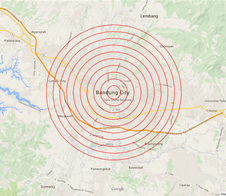
\includegraphics[scale=1]{Gambar/classificationmap.jpg}
\caption[\textsl{Classification} pada daerah Bandung]{\textsl{Classification} pada daerah Bandung} 
\end{figure}

Penentuan \textsl{classification} tersebut berdasarkan perkiraaan titik pusat yang sudah ditentukan, yaitu -6.92036,107.60500 dalam latitude dan longitude. Untuk mencari nilai rusuk dari lingkaran tersebut, maka akan diambil nilai titik kedua dari sisi lingkaran tersebut. Nilai sisi yang dipilih adalah -6.92036,107.67023 dalam latitude dan longitude. Maka untuk mendapatkan nilai rusuk dari lingkaran dapat diperoleh dengan cara menghitung \textsl{euclidean} dari kedua titik tersebut.

\begin{displaymath}
	r = \sqrt{(-6.92036 - (-6.92036))^{2} + (107.60500 - 107.67023)^{2}}
	r = 0.06523
\end{displaymath}

Dari perhitungan tersebut, maka dapat disimpulkan jika suatu nilai latitude dan longitude yang dihitung perbedaan jaraknya dengan titik pusat yang sudah ditentukan dan diperoleh nilainya kurang dari 0.06523, dapat dikatakan bahwa lokasinya berada di Bandung. Jika jaraknya lebih besar dari 0.06523, maka lokasinya berada di luar Bandung.

Nilai jarak dari lokasi keberangkatan terhadap titik pusat dan lokasi tujuan terhadap titik pusat, dapat dijadikan acuan untuk menentukan apakah \textsl{user} tersebut menuju daerah Bandung atau keluar dari Bandung. Kondisi yang menentukan apakah \textsl{user} menuju Bandung yaitu, jika jarak dari lokasi keberangkatan dengan titik pusat lebih besar daripada 0.06523 (dari luar Bandung) dan jarak dari lokasi tujuan dengan titik pusat lebih kecil dari 0.06523 (di dalam Bandung), maka dapat ditentukan bahwa \textsl{user} tersebut menuju Bandung.

Maka dari itu, nilai latitude dan longitude dari lokasi keberangkatan dan tujuan akan dibuang dan diganti oleh atribut menujuBandung dengan tipe data \textsl{integer}. Jika isi dari atribut tersebut bernilai 1, maka \textsl{user} tersebut menuju Bandung sedangkan nilai 0 bearti \textsl{user} tidak menuju Bandung, dan jika nilai atribut tersebut adalah 2, maka \textsl{user} tersebut memiliki lokasi keberangkatan dan tujuan di dalam Bandung. Contoh hasil data setelah dilakukan \textsl{transformation} terhadap latitude dan longitude terdapat pada tabel 3.3.

\begin{table}[h]
\caption{Contoh hasil data transformasi latitude longitude}
\begin{longtable}{|l|l|l|l|l|l|l|}
\hline
\textbf{Tanggal}	& \textbf{Bulan}	& \textbf{Tahun} 	& \textbf{Hari} & \textbf{Jam}	& \textbf{Menit} & \textbf{MenujuBandung} \\ \hline
01				         	& 02								& 2014						& Sabtu         & 00         	& 11						 & 2                    \\ \hline
01				         	& 02								& 2014						& Sabtu         & 00         	& 13						 & 1        					  \\ \hline
01				          & 02								& 2014						& Sabtu         & 00         	& 16						 & 1       							\\ \hline
01				          & 02								& 2014						& Sabtu         & 00         	& 18						 & 0         						\\ \hline
01				          & 02								& 2014						& Sabtu         & 00         	& 25						 & 1          					\\ \hline
01				          & 02								& 2014						& Sabtu         & 00         	& 27						 & 2      							\\ \hline
01				          & 02								& 2014						& Sabtu         & 00         	& 28						 & 0       							\\ \hline
\end{longtable}
\end{table} 


\section{Analisis Perangkat Lunak}
Agar analisis pola dari lokasi keberangkatan dan tujuan dari data \textsl{log} histori lebih mudah, maka akan dibangun sebuah perangkat lunak yang dapat melakukan proses \textsl{data mining} dengan menggunakan teknik ID3 dan C4.5, serta dapat melakukan visualisasi hasil dari \textsl{data mining} yang diperoleh setelah proses dijalankan yaitu perangkat lunak \textsl{data mining log} histori KIRI. 

Perangkat lunak yang akan dibangun akan berbasis desktop dan menggunakan bahasa pemograman java. Pada subbab ini akan dibahas spesifikasi kebutuhan funsional, pemodelan perangkat lunak, diagram \textsl{use case}, skenario, diagram kelas dari Perangkat Lunak yang akan dibangun.

\subsubsection{Spesifikasi Kebutuhan Fungsional Perangkat Lunak \textsl{Data Mining log} Histori KIRI}
Spesifikasi kebutuhan perangkat lunak yang akan dibangun untuk melakukan \textsl{data mining log} histori KIRI yang sesuai yang diharapkan adalah
\begin{enumerate}
	\item Dapat menerima dan membaca input text yang sudah disiapkan
	\item Dapat melakukan \textsl{preprocessing} data sesuai dengan yang dijelaskan pada bab analisis data
	\item Dapat melakukan proses \textsl{data mining}, ID3 dan C4.5
	\item Dapat melakukan visualisasi hasil dari \textsl{data mining} yang diperoleh
\end{enumerate}

\subsubsection{Pemodelan Perangkat Lunak \textsl{Data Mining Log} Histori KIRI}
Perangkat lunak \textsl{data mining log} histori KIRI akan mendapat input data text dengan format .txt. Setelah program mendapatkan input dan user menekan tombol proses, maka data tersebut akan diubah terlebih dahulu sesuai pada bab analisis data(bab 3.1) dengan melakukan proses \textsl{data transform} dan menghasilkan data dengan format seperti pada tabel 3.2.

Program akan melakukan tahap \textsl{data mining} dengan menggunakan teknik ID3 atau C4.5 sesuai dengan permintaan \textsl{user}. Setelah proses \textsl{data mining} selesai dilakukan, program akan melakukan \textsl{visualisasi decision tree} dan nilai klasifikasi yang diperoleh.  

\subsubsection{Pemodelan Data pada Perangkat Lunak \textsl{Data Mining Log} Histori KIRI}
Karena data yang diperoleh sudah dalam bentuk excel, maka pada penelitian ini, tidak akan menggunakan sistem database. Untuk mempermudah penelitian, data-data pada excel akan dipindahkan ke data text dengan format .txt. Isi dari file txt tersebut merupakan nilai dari atribut \textsl{timestamp}(UTC) dan \textsl{additionalData} yang dipisahkan dengan spasi. Hal ini dapat dilakukan dengan menggunakan fungsi \textsl{CONCATENATE} dari excel untuk membuat format sesuai yang diharapkan kemudian melakukan \textsl{copy} pada kolom \textsl{CONCATENATE} lalu \textsl{paste} pada file txt yang masih kosong. Contoh data input untuk perangkat lunak \textsl{data mining log} histori KIRI adalah

2/1/2014 0:11 -6.8972513,107.6385574/-6.91358,107.62718/1

2/1/2014 0:13 -6.8972513,107.6385574/-6.91358,107.62718/1

2/1/2014 0:16 -6.90598,107.59714/-6.90855,107.61082/1

Setelah dipindahkan ke dalam format .txt, maka data sudah siap untuk menjadi input perangkat lunak \textsl{data mining log} histori KIRI.

Ketika tombol proses ditekan, maka data tersebut akan diproses. Proses yang pertama yang akan dilakukan adalah melakukan \textsl{load} data dari file. Setelah data didapat, akan dilakukan proses \textsl{transform} untuk setiap baris yang ada. Proses \textsl{transform} tersebut memiliki tahap sebagai berikut:
\begin{enumerate}
	\item Mengambil nilai string pada baris tersebut
	\item Memecah nilai string yang didapat dengan spasi sebagai tanda pemisah, maka akan terdapat tiga nilai, yaitu tanggal, jam, dan \textsl{additionalData}
	\item Pada nilai tanggal, dilakukan pemecahan nilai string dengan garis miring sebagai tanda pemisah, maka akan diperoleh tiga nilai yaitu bulan, tanggal, dan tahun
	\item Pada nilai jam, dilakukan pemecahan nilai string dengan titik dua sebagai tanda pemisah, maka akan diperoleh dua nilai yaitu jam dan menit
	\item Pada \textsl{additionalData}, dilakukan pemecahan nilai string dengan garis miring sebagai tanda pemisah, maka akan diperoleh tiga nilai yaitu lokasi awal, lokasi tujuan, dan banyak jalur
	\item Mengubah waktu dari UTC menjadi GMT+8
	\item Mencari hari dengan memanfaatkan nilai tanggal, bulan, dan tahun serta kelas \textsl{calendar}
	\item menggabungkan nilai-nilai tersebut ke dalam dua array, yaitu array dengan tipe int (dengan nilai tanggal, bulan, tahun, jam, dan menit) dan array double (dengan nilai l sesuai dengan urutan yang diharapkan
\end{enumerate}

setelah proses \textsl{transform} berhasil dilaksanakan, maka data sudah siap untuk dijadikan nilai input untuk proses data mining pada perangkat lunak \textsl{data mining log} histori KIRI.

\subsubsection{Pemodelan Fungsi pada Perangkat Lunak \textsl{Data Mining Log} Histori KIRI}
Setelah \textsl{preprocessing} data selesai dilaksanakan, maka program akan menjalankan proses \textsl{data mining}. Proses tersebut memiliki tahap sebagai berikut
\begin{enumerate}
	\item Program akan menjalankan algoritma pembuat \textsl{decision tree} yang terdapat pada \ref{method_pohon_keputusan}
	\item Program akan menampilkan \textsl{decision tree}
\end{enumerate}  

Pada tahap pertama, isi method pada \textsl{attribute_selection_method} akan memiliki tahap proses sebagai berikut
\begin{enumerate}
	\item Program akan menghitung nilai entropy \textsl{class}
	\item Program akan menghitung nilai entropy dan mendapatkan nilai \textsl{gain info} untuk setiap atribut pada \textsl{attribute_list}
	\item Jika \textsl{user} memilih untuk menggunakan algoritma C4.5, maka program akan menghitung \textsl{splitInfo} dan menghitung \textsl{gainRasio}
	\item Program akan memilih atribut yang terbaik untuk dijadikan \textsl{node} (jika ID3 maka nilai \textsl{gainInfo} yang akan digunakan untuk memilih atribut, jika C4.5 maka nilai \textsl{gain Rasio} yang akan digunakan untuk memilih atribut)
	\item Program akan mengembalikan \textsl{node} yang dipilih berserta nilai tuple yang terdapat pada cabang masing-masing
\end{enumerate}

\subsection{Diagram \textsl{Use Case} Perangkat Lunak}
\subsection{Diagram kelas Perangkat Lunak}


















